\documentclass[tikz,border=8pt]{standalone}
\usepackage[scaled=0.95]{helvet}
\renewcommand{\familydefault}{\sfdefault}
\usepackage{tikz}
\usetikzlibrary{circuits.logic.US,positioning}
\definecolor{TEJNavy}{HTML}{1E2B55}
\definecolor{TEJBlue}{HTML}{1769AA}
\tikzset{
  every path/.style={draw=TEJNavy,line width=1.05pt},
  twogate/.style={draw,logic gate inputs=nn,scale=1.45},
  onegate/.style={draw,logic gate inputs=n,scale=1.45},
  gatename/.style={font=\bfseries\Large,text=TEJBlue},
  pinlabel/.style={font=\large,text=TEJNavy}
}
\newcommand{\twogate}[3]{%
  \node[#1,twogate] (#2) at #3 {};
  \draw (#2.input 1) -- ++(-0.65,0) node[left,pinlabel] {$A$};
  \draw (#2.input 2) -- ++(-0.65,0) node[left,pinlabel] {$B$};
  \draw (#2.output) -- ++(0.65,0) node[right,pinlabel] {$Y$};
}
\begin{document}
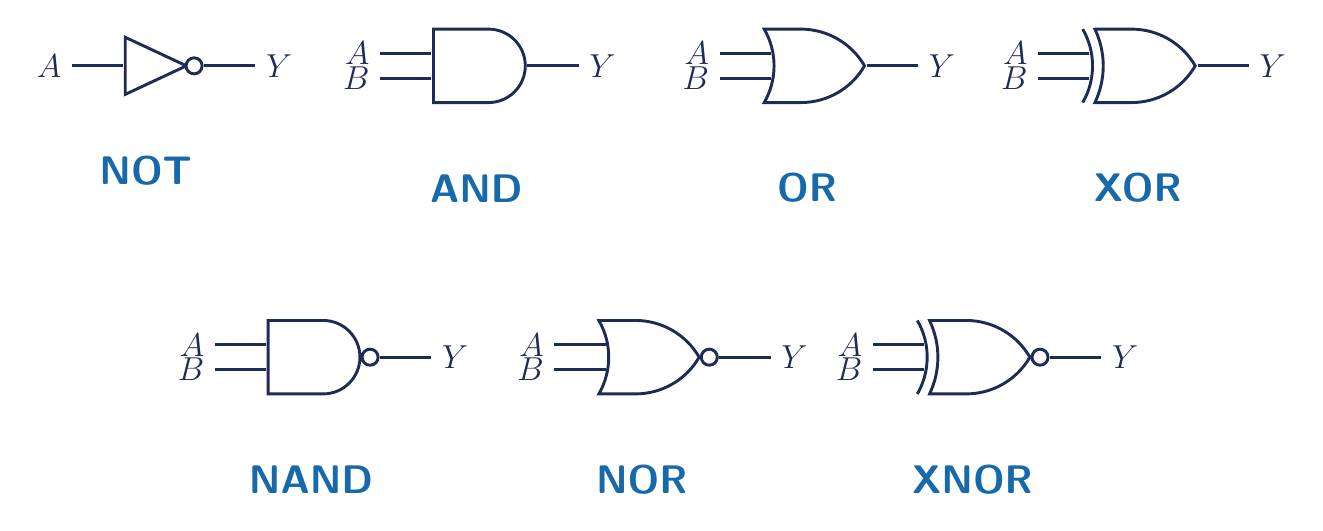
\begin{tikzpicture}
  \node[not gate US,onegate] (not) at (0,3.7) {};
  \draw (not.input) -- ++(-0.65,0) node[left,pinlabel] {$A$};
  \draw (not.output) -- ++(0.65,0) node[right,pinlabel] {$Y$};
  \node[gatename,below=0.75cm of not] {NOT};

  \twogate{and gate US}{and}{(4.2,3.7)}
  \node[gatename,below=0.75cm of and] {AND};
  \twogate{or gate US}{or}{(8.4,3.7)}
  \node[gatename,below=0.75cm of or] {OR};
  \twogate{xor gate US}{xor}{(12.6,3.7)}
  \node[gatename,below=0.75cm of xor] {XOR};

  \twogate{nand gate US}{nand}{(2.1,0)}
  \node[gatename,below=0.75cm of nand] {NAND};
  \twogate{nor gate US}{nor}{(6.3,0)}
  \node[gatename,below=0.75cm of nor] {NOR};
  \twogate{xnor gate US}{xnor}{(10.5,0)}
  \node[gatename,below=0.75cm of xnor] {XNOR};
\end{tikzpicture}
\end{document}
